\documentclass[12pt, a4paper]{article}

% --- PACKAGES ---
\usepackage[utf8]{inputenc} % Input encoding
\usepackage[T1]{fontenc}    % Font encoding
\usepackage[czech]{babel}   % Czech language support
\usepackage{geometry}       % Page layout (adjust margins if needed)
\geometry{a4paper, margin=2.5cm}
\usepackage{graphicx}       % For including images (if needed later for screenshots)
\usepackage{amsmath}        % For math environments
\usepackage{amssymb}        % For math symbols
\usepackage[hyphens]{url}   % For handling URLs and file paths with line breaks (Load ONCE before hyperref)
\usepackage{enumitem}       % For customizing lists
\usepackage[patch=none]{microtype}  % Improves typography, disable problematic patches
\usepackage{listings}
\lstset{
    breaklines=true,
    basicstyle=\ttfamily\small,
    columns=flexible,
    inputencoding=utf8,
    extendedchars=true,
    literate={á}{{\'a}}1 {č}{{\v{c}}}1 {ě}{{\v{e}}}1 {í}{{\'i}}1 {š}{{\v{s}}}1 {ť}{{\v{t}}}1 {ů}{{\r{u}}}1 {ž}{{\v{z}}}1
}

% Load hyperref towards the end
\usepackage{hyperref}       % For clickable links and table of contents
\hypersetup{
    colorlinks=true,
    linkcolor=blue,
    filecolor=magenta,
    urlcolor=cyan,
    pdftitle={Seminární práce DBS2 - ActiveLife},
    pdfpagemode=UseOutlines,
    breaklinks=true % Allows links to break across lines
}


% --- DOCUMENT INFORMATION ---
\title{Seminární práce z předmětu Databázové systémy 2 \\ Sportovní centrum ``ActiveLife''}
\author{Členové pracovního týmu: \\  Jakub Doležal, Jakub Kyzr, Václav Havelka}
\date{V Hradci Králové \\ dne \today} % Or set a specific date: dne 20. dubna 2025

% --- BEGIN DOCUMENT ---
\begin{document}

% --- TITLE PAGE ---
\begin{titlepage}
    \centering
    \vspace*{1cm}
    {\Large UNIVERZITA HRADEC KRÁLOVÉ \\ FAKULTA INFORMATIKY A MANAGEMENTU}
    \vspace*{3cm}

    {\Huge\bfseries Aplikace pro sportovní centrum ,,ActiveLife``} % As per the template, though seems like a placeholder
    \vspace*{3cm}

    {\Large Seminární práce z předmětu Databázové systémy 2}
    \vspace*{1cm}

    {\large Členové pracovního týmu DataForge:} \\
    \vspace*{0.5cm}
    Jakub Doležal, Jakub Kyzr, Václav Havelka % Placeholder for team members

    \vfill % Pushes the date to the bottom

    {V Hradci Králové \\ dne 20. dubna 2025} % Example date

\end{titlepage}

% --- TABLE OF CONTENTS ---
\tableofcontents
\newpage

% --- CHAPTERS/SECTIONS FROM MARKDOWN ---

% ... (Rest of the document remains the same as the previous version) ...
% Sections: Úvod, Zadání, Uživatelská dokumentace, Programová dokumentace, Závěr, Přílohy
% Using \url{...} for URLs and \path{...} for file paths

\section{Úvod}
\label{sec:uvod}

Cílem projektu je vytvoření moderní databázové aplikace pro sportovní centrum ``ActiveLife'', která zajistí efektivní správu rezervací sportovišť a aktivit. Nový systém nahradí dosavadní, převážně manuální řešení, které již nedostačuje rostoucím požadavkům centra. Sportovní centrum nabízí široké spektrum aktivit a dosavadní IT řešení založené na jednoduché evidenci je neflexibilní a pomalé. Nová aplikace má za cíl zefektivnit provoz, usnadnit správu informací a zlepšit uživatelskou zkušenost.

\section{Zadání}
\label{sec:zadani}

Aplikace bude nasazena v prostředí sportovního centra ``ActiveLife'', které potřebuje nahradit stávající manuální systém rezervací moderním databázovým řešením. Požadavky na nový systém zahrnují:

\begin{itemize}
    \item \textbf{Evidence a správa dat:} Záznamy o uživatelích (návštěvnících), sportovištích, aktivitách, rezervacích v časových slotech (včetně storna a úprav) a zaměstnancích (včetně směn).
    \item \textbf{Vstupy:} Uživatelské formuláře pro registraci, přihlášení, vytváření a úpravu rezervací, zadávání aktivit a cen.
    \item \textbf{Výstupy:} Reporty o využití sportovišť, seznam rezervací pro uživatele, statistiky pro plánování a marketing.
    \item \textbf{Uživatelské role:} Běžný uživatel (správa vlastních rezervací), Zaměstnanec (správa rezervací, provozní informace), Správce centra (plná správa systému, cen, reportů).
    \item \textbf{Technické požadavky:} Relační databáze (PostgreSQL), intuitivní a responzivní uživatelské rozhraní (Next.js, React, shadcn/ui, Tailwind CSS), zabezpečení (šifrovaná komunikace, NextAuth.js), verzování (Git), kontejnerizace (Docker).
\end{itemize}

\section{Uživatelská dokumentace}
\label{sec:uzivatelska_dokumentace}

\subsection{Základní popis používané aplikace}
\label{subsec:zakladni_popis}

Tato aplikace slouží ke komplexní správě rezervací sportovního centra ``ActiveLife''. Umožňuje uživatelům prohlížet dostupná sportoviště a aktivity, vytvářet a spravovat své rezervace online. Zaměstnancům a správcům centra poskytuje nástroje pro efektivní řízení provozu, správu kapacit, cen a generování reportů. Cílem je zjednodušit rezervační proces a poskytnout přehledné informace všem zúčastněným stranám.

\subsection{Instalace}
\label{subsec:instalace}

Aplikace je navržena pro spuštění pomocí Dockeru a Docker Compose.

\begin{enumerate}
    \item Naklonujte repozitář projektu.
    \item V kořenovém adresáři projektu spusťte příkaz \texttt{docker-compose up -d}. Tím se spustí potřebné služby (aplikační server, databáze) v kontejnerech.
    \item Databáze se inicializuje automaticky včetně migrací a základních dat (seed).
    \item Pro lokální vývoj bez Dockeru je potřeba mít nainstalovaný Node.js (včetně PNPM) a PostgreSQL. Závislosti se instalují pomocí \texttt{pnpm install}. Databáze se nastaví pomocí Prisma migrací (\texttt{pnpm prisma migrate dev}) a seedování (\texttt{pnpm prisma db seed}).
    \item Aplikace bude dostupná na adrese \url{http://localhost:3000} (nebo dle konfigurace).
\end{enumerate}

\subsection{Přístupová oprávnění}
\label{subsec:pristupova_opravneni}

Aplikace využívá systém rolí pro řízení přístupu k funkcím. Existují tři základní role:

\begin{itemize}
    \item \textbf{Běžný uživatel:} Může se registrovat, přihlásit, spravovat svůj profil, prohlížet sportoviště/aktivity a vytvářet/spravovat vlastní rezervace.
    \item \textbf{Zaměstnanec:} Má práva běžného uživatele a navíc může spravovat všechny rezervace, zadávat rezervace manuálně a vidět přehledy směn.
    \item \textbf{Správce centra:} Má nejvyšší oprávnění, včetně všech práv zaměstnance, a navíc může spravovat uživatele, role, sportoviště, aktivity, ceny a generovat systémové reporty.
\end{itemize}

Pro testování jsou k dispozici následující ukázkové účty:

\begin{itemize}
    \item Uživatel: \texttt{petr.svoboda@example.com}, Heslo: \texttt{user123}
    \item Zaměstnanec: \texttt{zamestnanec@activelife.cz}, Heslo: \texttt{zam123}
    \item Správce: \texttt{admin@activelife.cz}, Heslo: \texttt{admin123}
\end{itemize}

\subsection{Použití aplikace}
\label{subsec:pouziti_aplikace}

Aplikace je rozdělena do několika hlavních modulů dle uživatelských rolí:

\begin{itemize}
    \item \textbf{Veřejná část:} Úvodní obrazovka, katalog sportovišť a aktivit, registrační a přihlašovací formulář.
    \item \textbf{Modul pro běžné uživatele:} Osobní účet, přehled vlastních rezervací, rezervační systém (kalendář, výběr slotů), historie.
    \item \textbf{Modul pro zaměstnance:} Správa denních rezervací, přehled obsazenosti, manuální zadávání rezervací, správa směn.
    \item \textbf{Modul pro správce centra:} Správa uživatelů a rolí, správa sportovišť a aktivit, cenová politika, systémová nastavení, generování reportů, plánování směn.
\end{itemize}

Základní kroky pro rezervaci:

\begin{enumerate}
    \item Přihlaste se nebo se zaregistrujte.
    \item Přejděte do sekce rezervací nebo katalogu sportovišť/aktivit.
    \item Vyberte požadované sportoviště/aktivitu, datum a časový slot.
    \item Potvrďte rezervaci.
\end{enumerate}

\section{Programová dokumentace}
\label{sec:programova_dokumentace}

\subsection{Datová část}
\label{subsec:datova_cast}

Datová část aplikace je postavena na relační databázi PostgreSQL a spravována pomocí Prisma ORM. Model zahrnuje entity pro uživatele, role, zaměstnance, sportoviště, aktivity, časové sloty, rezervace, směny a další.

\subsubsection{Analýza}
\label{subsubsec:analyza}

Datový model byl navržen na základě analýzy požadavků sportovního centra ,,ActiveLife``. Cílem bylo vytvořit flexibilní a škálovatelnou strukturu pro správu rezervací.

\paragraph{Klíčové entity a vztahy}
Entitně-vztahový diagram (ERD) znázorňuje následující klíčové entity a jejich vztahy:

\begin{itemize}
    \item \textbf{Uživatelé a role:} User-Reservation (1:N), User-Role (N:1)
    \item \textbf{Sportoviště:} Facility-TimeSlot (1:N), Facility-Activity (M:N)
    \item \textbf{Rezervace:} TimeSlot-Reservation (1:N)
    \item \textbf{Zaměstnanci:} Employee-EmployeeShift (1:N)
\end{itemize}

\paragraph{Uživatelské rozhraní}
Aplikace je navržena jako responzivní webová aplikace s moduly pro různé role uživatelů.

\begin{figure}[htbp]
    \centering
    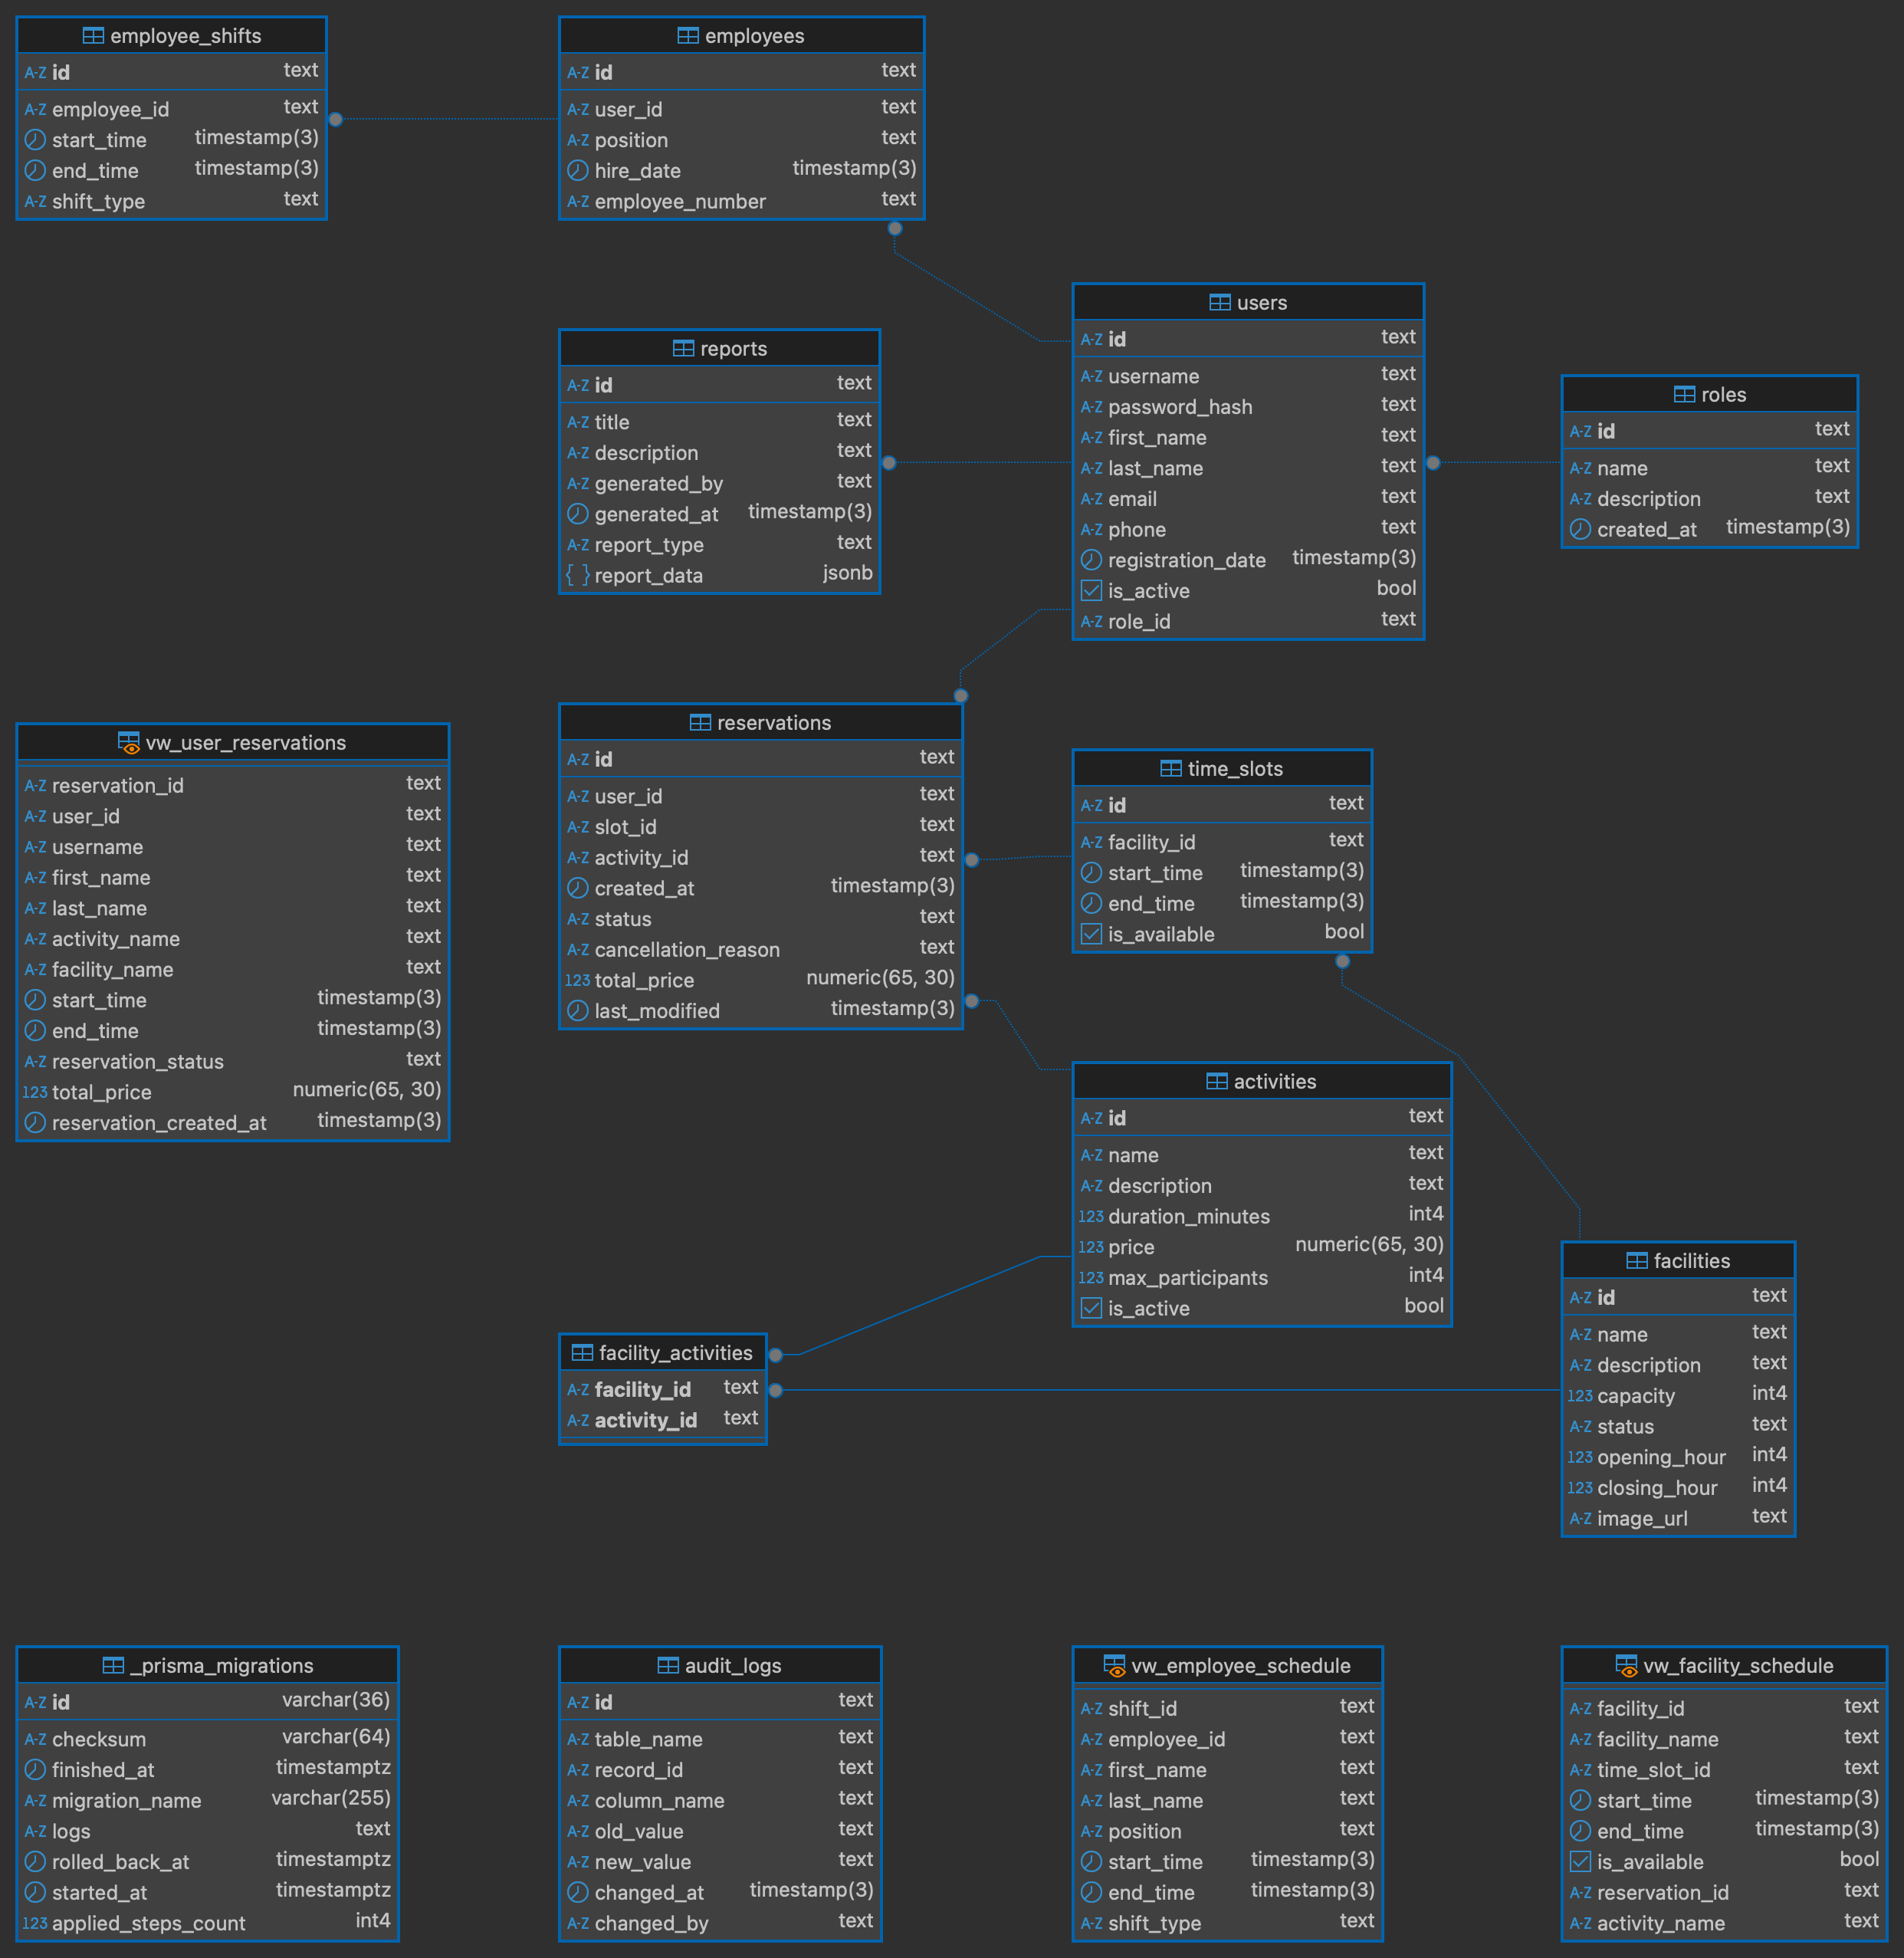
\includegraphics[width=0.8\textwidth]{erd_diagram.png}
    \caption{Entitně-vztahový diagram (ERD) hlavních entit systému}
    \label{fig:erd}
\end{figure}

\subsubsection{Fyzický model dat}
\label{subsubsec:fyzicky_model}

Fyzický model dat je definován v souboru \path{prisma/schema.prisma} a v migračních SQL skriptech. Tento model zahrnuje definice všech tabulek, jejich polí, datových typů, relací (cizích klíčů) a indexů. Prisma zajišťuje mapování mezi tímto schématem a skutečnou strukturou databáze PostgreSQL.

Klíčové tabulky zahrnují
\texttt{User},
\texttt{Role},
\texttt{Facility},
\texttt{Activity},
\texttt{Time\-Slot},
\texttt{Reservation},
\texttt{Employee\-Shift}
a také spojovací tabulky pro M:N vztahy. Například propojení sportovišť a aktivit je realizováno pomocí tabulky \texttt{facility\_activities}.

\paragraph{Ukázka SQL definice spojovací tabulky:}
\begin{lstlisting}
CREATE TABLE facility_activities (
  facility_id text NOT NULL,
  activity_id text NOT NULL,
  CONSTRAINT facility_activities_pkey PRIMARY KEY (facility_id, activity_id),
  CONSTRAINT facility_activities_activity_id_fkey FOREIGN KEY (activity_id) REFERENCES activities(id) ON DELETE CASCADE ON UPDATE CASCADE,
  CONSTRAINT facility_activities_facility_id_fkey FOREIGN KEY (facility_id) REFERENCES facilities(id) ON DELETE CASCADE ON UPDATE CASCADE
);
\end{lstlisting}

Datový slovník s popisem jednotlivých tabulek a sloupců je implicitně obsažen v \texttt{schema.prisma}.

\subsubsection{Číselníky}
\label{subsubsec:ciselniky}

Projekt využívá následující číselníky:

\begin{itemize}
    \item \textbf{Role:} Tabulka \texttt{Role} definuje možné uživatelské role v systému:
    \begin{itemize}
        \item \texttt{'ADMIN'} -- Administrátor s plným přístupem
        \item \texttt{'EMPLOYEE'} -- Zaměstnanec s provozním přístupem
        \item \texttt{'USER'} -- Běžný uživatel se základním přístupem
    \end{itemize}
    Zdroj: Definováno v \path{prisma/seed/seed-users.ts}
    
    \item \textbf{Status sportoviště:} Sloupec \texttt{status} v tabulce \texttt{Facility}:
    \begin{itemize}
        \item \texttt{'ACTIVE'} -- Sportoviště je aktivní a dostupné
        \item \texttt{'MAINTENANCE'} -- Sportoviště je v údržbě
        \item \texttt{'CLOSED'} -- Sportoviště je uzavřeno
    \end{itemize}
    Zdroj: Definováno v \path{prisma/seed/seed-sport-facilities.ts}
    
    \item \textbf{Status rezervace:} Sloupec \texttt{status} v tabulce \texttt{Reservation}:
    \begin{itemize}
        \item \texttt{'confirmed'} -- Potvrzená rezervace
        \item \texttt{'pending'} -- Čekající na potvrzení
        \item \texttt{'cancelled'} -- Zrušená rezervace
    \end{itemize}
    Zdroj: Definováno v \path{prisma/seed/seed-reservations.ts}
    
    \item \textbf{Typ směny:} Sloupec \texttt{shift\_type} v tabulce \texttt{EmployeeShift}:
    \begin{itemize}
        \item \texttt{'Ranní'} -- Ranní směna (typicky 8:00-16:00)
        \item \texttt{'Odpolední'} -- Odpolední směna (typicky 14:00-22:00)
    \end{itemize}
    Zdroj: Definováno v \path{prisma/seed/seed-employee-shifts.ts}
\end{itemize}

Všechny číselníky jsou implementovány jako textové sloupce v databázi a jejich hodnoty jsou validovány na aplikační úrovni pomocí TypeScript typů a Zod schémat.

\subsubsection{Pohledy}
\label{subsubsec:pohledy}

V databázi jsou definovány následující pohledy pro zjednodušení dotazů a reportingu (definované v \path{prisma/migrations/20250420125507_add_initial_views/migration.sql}):

\begin{itemize}
    \item \texttt{vw\_user\_reservations}: Zobrazuje detailní informace o rezervacích včetně údajů o uživateli, aktivitě a sportovišti.
    \item \texttt{vw\_facility\_schedule}: Poskytuje přehled rozvrhu sportovišť včetně obsazenosti a plánovaných aktivit.
    \item \texttt{vw\_employee\_schedule}: Zobrazuje rozpis směn zaměstnanců s jejich osobními údaji.
\end{itemize}

\paragraph{vw\_user\_reservations:}
\begin{lstlisting}
CREATE VIEW vw_user_reservations AS
SELECT
    r.id as reservation_id,
    u.id as user_id,
    u.username,
    u.first_name,
    u.last_name,
    a.name as activity_name,
    f.name as facility_name,
    ts.start_time,
    ts.end_time,
    r.status as reservation_status,
    r.total_price,
    r.created_at as reservation_created_at
FROM reservations r
JOIN users u ON r.user_id = u.id
JOIN activities a ON r.activity_id = a.id
JOIN time_slots ts ON r.slot_id = ts.id
JOIN facilities f ON ts.facility_id = f.id;
\end{lstlisting}

\paragraph{vw\_facility\_schedule:}
\begin{lstlisting}
CREATE VIEW vw_facility_schedule AS
SELECT
    f.id as facility_id,
    f.name as facility_name,
    ts.id as time_slot_id,
    ts.start_time,
    ts.end_time,
    ts.is_available,
    r.id as reservation_id,
    a.name as activity_name
FROM facilities f
JOIN time_slots ts ON f.id = ts.facility_id
LEFT JOIN reservations r ON ts.id = r.slot_id AND r.status != 'cancelled'
LEFT JOIN activities a ON r.activity_id = a.id;
\end{lstlisting}

\paragraph{vw\_employee\_schedule:}
\begin{lstlisting}
CREATE VIEW vw_employee_schedule AS
SELECT
    es.id as shift_id,
    e.id as employee_id,
    u.first_name,
    u.last_name,
    e.position,
    es.start_time,
    es.end_time,
    es.shift_type
FROM employee_shifts es
JOIN employees e ON es.employee_id = e.id
JOIN users u ON e.user_id = u.id;
\end{lstlisting}

\subsubsection{Funkce}
\label{subsubsec:funkce}

Projekt využívá následující databázové funkce (definované v \path{prisma/migrations/20250420131104_add_db_functions/migration.sql}):

\begin{itemize}
    \item \texttt{calculate\_facility\_revenue}: Kalkuluje celkové příjmy pro dané sportoviště v zadaném období z potvrzených rezervací.
    \item \texttt{check\_user\_active\_reservations}: Vrací počet aktivních (budoucích potvrzených nebo čekajících) rezervací pro daného uživatele.
    \item \texttt{get\_facility\_availability\_summary}: Poskytuje textový souhrn dostupných vs. celkových časových slotů pro dané sportoviště a den.
\end{itemize}

\paragraph{calculate\_facility\_revenue:}
\begin{lstlisting}
CREATE OR REPLACE FUNCTION calculate_facility_revenue(
    p_facility_id TEXT,
    p_start_date DATE,
    p_end_date DATE
)
RETURNS DECIMAL AS $$
DECLARE
    total_revenue DECIMAL;
BEGIN
    SELECT COALESCE(SUM(r.total_price), 0.00)
    INTO total_revenue
    FROM reservations r
    JOIN time_slots ts ON r.slot_id = ts.id
    WHERE ts.facility_id = p_facility_id
      AND r.status = 'confirmed'
      AND ts.start_time >= p_start_date::timestamp
      AND ts.start_time < (p_end_date + interval '1 day')::timestamp;

    RETURN total_revenue;
END;
$$ LANGUAGE plpgsql;
\end{lstlisting}

\paragraph{check\_user\_active\_reservations:}
\begin{lstlisting}
CREATE OR REPLACE FUNCTION check_user_active_reservations(
    p_user_id TEXT
)
RETURNS INTEGER AS $$
DECLARE
    active_count INTEGER;
BEGIN
    SELECT COUNT(*)
    INTO active_count
    FROM reservations r
    JOIN time_slots ts ON r.slot_id = ts.id
    WHERE r.user_id = p_user_id
      AND r.status IN ('confirmed', 'pending')
      AND ts.start_time >= NOW();

    RETURN active_count;
END;
$$ LANGUAGE plpgsql;
\end{lstlisting}

\paragraph{get\_facility\_availability\_summary:}
\begin{lstlisting}
CREATE OR REPLACE FUNCTION get_facility_availability_summary(
    p_facility_id TEXT,
    p_check_date DATE
)
RETURNS TEXT AS $$
DECLARE
    facility_name TEXT;
    total_slots INTEGER;
    available_slots INTEGER;
    summary TEXT;
BEGIN
    SELECT name INTO facility_name FROM facilities WHERE id = p_facility_id;

    IF NOT FOUND THEN
        RETURN 'Sportoviste nenalezeno.';
    END IF;

    SELECT COUNT(*)
    INTO total_slots
    FROM time_slots ts
    WHERE ts.facility_id = p_facility_id
      AND ts.start_time >= p_check_date::timestamp
      AND ts.start_time < (p_check_date + interval '1 day')::timestamp;

    SELECT COUNT(*)
    INTO available_slots
    FROM time_slots ts
    WHERE ts.facility_id = p_facility_id
      AND ts.start_time >= p_check_date::timestamp
      AND ts.start_time < (p_check_date + interval '1 day')::timestamp
      AND ts.is_available = TRUE;

    summary := available_slots::TEXT || '/' || total_slots::TEXT || 
               ' slotu volnych dne ' || to_char(p_check_date, 'DD.MM.YYYY');

    RETURN summary;
END;
$$ LANGUAGE plpgsql;
\end{lstlisting}

Tyto funkce jsou volány z aplikace pomocí \texttt{prisma.\$queryRaw}.

\subsubsection{Uložené procedury}
\label{subsubsec:ulozene_procedury}

Projekt využívá následující uložené procedury (definované v \path{prisma/migrations/20250420132146_add_stored_procedures/migration.sql}):

\begin{itemize}
    \item \texttt{cancel\_reservation(p\_reservation\_id UUID, p\_cancellation\_reason TEXT)}: Aktualizuje status rezervace na \texttt{'CANCELLED'} a zaznamená důvod zrušení.
    \item \texttt{deactivate\_user(p\_user\_id UUID)}: Nastaví příznak \texttt{is\_active} uživatele na \texttt{false}. (Použito triggerem \texttt{trg\_user\_deactivation}).
    \item \texttt{assign\_employee\_shift(p\_employee\_id UUID, p\_start\_time TIMESTAMP WITH TIME ZONE, p\_end\_time TIMESTAMP WITH TIME ZONE, p\_shift\_type TEXT)}: Vloží novou pracovní směnu pro zaměstnance.
\end{itemize}
Tyto procedury jsou volány z aplikace pomocí \texttt{prisma.\$executeRaw} \\ nebo \texttt{prisma.\$executeRawUnsafe}.

\paragraph{cancel\_reservation:}
\begin{lstlisting}
CREATE OR REPLACE PROCEDURE cancel_reservation(
    p_reservation_id TEXT,
    p_cancellation_reason TEXT
)
LANGUAGE plpgsql
AS $$
BEGIN
    UPDATE reservations
    SET status = 'cancelled',
        cancellation_reason = p_cancellation_reason,
        last_modified = NOW()
    WHERE reservation_id = p_reservation_id;
END;
$$;
\end{lstlisting}

\paragraph{deactivate\_user:}
\begin{lstlisting}
CREATE OR REPLACE PROCEDURE deactivate_user(
    p_user_id TEXT
)
LANGUAGE plpgsql
AS $$
BEGIN
    UPDATE users
    SET is_active = false
    WHERE id = p_user_id;
END;
$$;
\end{lstlisting}

\paragraph{assign\_employee\_shift:}
\begin{lstlisting}
CREATE OR REPLACE PROCEDURE assign_employee_shift(
    p_employee_id TEXT,
    p_start_time TIMESTAMP WITH TIME ZONE,
    p_end_time TIMESTAMP WITH TIME ZONE,
    p_shift_type TEXT
)
LANGUAGE plpgsql
AS $$
BEGIN
    INSERT INTO employee_shifts (shift_id, employee_id, start_time, end_time, shift_type)
    VALUES (gen_random_uuid()::text, p_employee_id, p_start_time, p_end_time, p_shift_type);
END;
$$;
\end{lstlisting}

\subsubsection{Sekvence}
\label{subsubsec:sekvence}

Projekt nevyužívá explicitně definované sekvence pro generování číselných ID. Místo toho jsou primární klíče implementovány jako UUID, které jsou generovány následujícími způsoby:

\begin{itemize}
    \item Většina tabulek používá UUID generované pomocí Prisma \texttt{@default(uuid())} nebo přímo v PostgreSQL pomocí \texttt{gen\_random\_uuid()}.
    \item Tabulka \texttt{audit\_logs} používá \texttt{@default(dbgenerated("gen\_random\_uuid()"))} pro přímé generování UUID v databázi.
    \item V seed datech jsou UUID generována pomocí \texttt{randomUUID()} z Node.js crypto modulu.
\end{itemize}

Toto řešení bylo zvoleno pro zajištění globální unikátnosti identifikátorů napříč celou aplikací a pro usnadnění případné distribuce nebo replikace dat v budoucnu.

\subsection{Aplikace}
\label{subsec:aplikace}

Aplikační část je postavena na frameworku Next.js s využitím App Routeru. Frontend využívá React, TypeScript a komponentovou knihovnu shadcn/ui s Tailwind CSS pro stylování. Backendová logika je řešena pomocí API routes v Next.js a interaguje s databází přes Prisma ORM.

\subsubsection{Použité prostředí}
\label{subsubsec:pouzite_prostredi}

\begin{itemize}
    \item \textbf{Framework:} Next.js (v14+ s App Router)
    \item \textbf{Jazyk:} TypeScript
    \item \textbf{Frontend:} React (v18+), shadcn/ui, Tailwind CSS, Zustand (pro state management), React Hook Form (pro formuláře), Sonner (pro notifikace)
    \item \textbf{Backend (API Routes):} Node.js (runtime Next.js)
    \item \textbf{Databáze:} PostgreSQL (v15+)
    \item \textbf{ORM:} Prisma (v5+)
    \item \textbf{Autentizace/Autorizace:} NextAuth.js (v5+)
    \item \textbf{Package Manager:} PNPM
    \item \textbf{Kontejnerizace:} Docker, Docker Compose
    \item \textbf{Verzování:} Git
    \item \textbf{Linting/Formátování:} ESLint, Prettier
\end{itemize}

\subsubsection{Řízení uživatelských účtů}
\label{subsubsec:rizeni_uctu}

Správa uživatelských účtů a autentizace je řešena pomocí knihovny NextAuth.js. Při registraci se ukládají údaje uživatele do tabulky \texttt{User}, včetně hashe hesla (používá se bcrypt). Každý uživatel má přiřazenou roli (odkaz na tabulku \texttt{Role}), která určuje jeho oprávnění (Role-Based Access Control - RBAC). Middleware v Next.js (\path{src/middleware.ts}) a kontroly na úrovni API routes a serverových komponent ověřují autentizaci a autorizaci uživatele pro přístup k chráněným zdrojům a funkcím na základě jeho role.

\subsubsection{Moduly}
\label{subsubsec:moduly}

Aplikace je strukturována do modulů, které odpovídají hlavním funkčním oblastem a uživatelským rolím:

\begin{itemize}
    \item \textbf{Autentizace (\path{src/app/(auth)}):} Registrace, přihlášení, odhlášení a správa autentizace uživatelů.
    \item \textbf{Správa účtu (\path{src/app/app/account}):} Úprava profilu a nastavení uživatelského účtu.
    \item \textbf{Zaměstnanecký modul (\path{src/app/app/employee}):} Správa rezervací a směn pro zaměstnance.
    \item \textbf{Správa sportovišť (\path{src/app/app/facilities}):} Zobrazení seznamu, detailu, dostupnosti, vytváření a editace sportovišť.
    \item \textbf{Rezervace (\path{src/app/app/reservations}):} Vytváření a správa rezervací, přehled vlastních a všech rezervací.
    \item \textbf{Správa uživatelů (\path{src/app/app/users}):} Správa uživatelských účtů a jejich oprávnění.
    \item \textbf{API Routes (\path{src/app/api}):} Backend logika zahrnující:
        \begin{itemize}
            \item \path{/api/activities}: Správa sportovních aktivit
            \item \path{/api/auth}: Autentizační endpointy
            \item \path{/api/facilities}: CRUD operace pro sportoviště
            \item \path{/api/reservations}: Správa rezervací
            \item \path{/api/time-slots}: Správa časových slotů
            \item \path{/api/user}: Správa uživatelského profilu
        \end{itemize}
    \item \textbf{Komponenty (\path{src/components}):} Znovu použitelné UI komponenty:
        \begin{itemize}
            \item \path{auth/}: Komponenty pro autentizaci
            \item \path{facilities/}: Komponenty pro správu sportovišť
            \item \path{profile/}: Komponenty pro uživatelský profil
            \item \path{reservations/}: Komponenty pro rezervace
            \item \path{ui/}: Obecné UI komponenty postavené na shadcn/ui
            \item \path{users/}: Komponenty pro správu uživatelů
        \end{itemize}
    \item \textbf{Knihovny a utility (\path{src/lib}):} Sdílené funkce a konfigurace:
        \begin{itemize}
            \item Databázový klient (Prisma)
            \item TypeScript typy a rozhraní
            \item Utility funkce
            \item Konfigurace NextAuth.js
        \end{itemize}
    \item \textbf{Middleware (\path{src/middleware.ts}):} Implementace autentizace a autorizace na úrovni routování.
\end{itemize}

\subsubsection{Formuláře}
\label{subsubsec:formulare}

Aplikace využívá React Hook Form s Zod schématy pro validaci formulářů. Všechny formuláře jsou implementovány s důrazem na uživatelskou přívětivost a validaci dat. Klíčové formuláře zahrnují:

\begin{itemize}
    \item \textbf{Autentizační formuláře (\path{src/components/ui/auth-form.tsx}):}
        \begin{itemize}
            \item Přihlašovací formulář: Email (validace formátu), heslo (min. 6 znaků)
            \item Registrační formulář: Uživatelské jméno (3-20 znaků), jméno, příjmení, email, heslo, telefon (volitelný)
        \end{itemize}
    \item \textbf{Formulář pro správu sportovišť (\path{src/components/facilities/facility-form.tsx}):}
        \begin{itemize}
            \item Název (min. 3 znaky)
            \item Popis (volitelný)
            \item Kapacita (kladné číslo)
            \item Status (aktivní/v údržbě/uzavřeno)
            \item Otevírací a zavírací hodina (0-23, validace vzájemného vztahu)
            \item URL obrázku (volitelné, validace formátu URL)
        \end{itemize}
    \item \textbf{Formulář pro manuální rezervace (\path{src/components/reservations/ManualReservationDialog.tsx}):}
        \begin{itemize}
            \item Vyhledávání/výběr uživatele s možností vytvoření nového
            \item Výběr sportoviště a aktivity (dynamicky načítané)
            \item Výběr data a časového slotu
            \item Interní poznámky (volitelné)
            \item Komplexní validace dostupnosti a oprávnění
        \end{itemize}
    \item \textbf{Formuláře pro správu uživatelů:}
        \begin{itemize}
            \item Editace uživatele (\path{src/components/users/edit-user-form.tsx})
            \item Přidání uživatele (\path{src/components/users/add-user-form.tsx})
        \end{itemize}
    \item \textbf{Formuláře pro správu profilu:}
        \begin{itemize}
            \item Editace profilu (\path{src/components/profile/edit-profile-form.tsx})
            \item Změna hesla (\path{src/components/profile/change-password-form.tsx})
        \end{itemize}
\end{itemize}

Všechny formuláře implementují:
\begin{itemize}
    \item Validaci na straně klienta pomocí Zod schémat
    \item Okamžitou zpětnou vazbu při chybách
    \item Ošetření stavů načítání a chyb
    \item Notifikace o úspěchu/neúspěchu pomocí knihovny Sonner
    \item Responzivní design pomocí shadcn/ui komponent
    \item Přístupnost (ARIA atributy, klávesová ovladatelnost)
\end{itemize}

\subsubsection{Orientace ve zdrojovém kódu}
\label{subsubsec:orientace_kod}

Zdrojový kód projektu je organizován ve složce \path{src} a následuje konvence Next.js App Routeru:

\begin{itemize}
    \item \textbf{\path{src/app/}:} Hlavní složka aplikace.
        \begin{itemize}
            \item \path{(auth)/}: Route group pro autentizační stránky (login, register).
            \item \path{api/}: Backend API routes. Každá podsložka obvykle odpovídá entitě nebo funkční oblasti (např. \path{api/facilities}, \path{api/reservations}). Obsahuje \path{route.ts} soubory s handlery pro HTTP metody (GET, POST, PUT, DELETE).
            \item \path{app/}: Route group pro chráněné části aplikace dostupné po přihlášení.
                \begin{itemize}
                    \item \path{layout.tsx}: Hlavní layout pro přihlášené uživatele.
                    \item \path{page.tsx}: Výchozí stránka po přihlášení (dashboard).
                    \item Podsložky odpovídají hlavním sekcím aplikace (\path{facilities}, \path{reservations}, \path{account}, \path{users}). Stránky jsou definovány v \path{page.tsx}, specifické layouty v \path{layout.tsx}. Dynamické segmenty (např. \path{[id]}) slouží pro detailní stránky.
                \end{itemize}
        \end{itemize}
    \item \textbf{\path{src/components/}:} Znovu použitelné React komponenty.
        \begin{itemize}
            \item \path{ui/}: Komponenty z shadcn/ui (generované CLI).
            \item \path{auth/}, \path{facilities/}, \path{profile/}, etc.: Aplikačně specifické komponenty.
        \end{itemize}
    \item \textbf{\path{src/lib/}:} Sdílené knihovny, utility a typy.
        \begin{itemize}
            \item \path{db.ts}: Inicializace a export Prisma klienta.
            \item \path{types.ts}: Definice TypeScript typů a rozhraní.
            \item \path{utils.ts}: Pomocné funkce.
            \item \path{auth.ts}: Konfigurace NextAuth.js.
        \end{itemize}
    \item \textbf{\path{src/hooks/}:} Vlastní React hooky.
    \item \textbf{\path{src/providers/}:} React context providers (např. pro session, theme).
    \item \textbf{\path{prisma/}:} Soubory související s Prisma ORM.
        \begin{itemize}
            \item \path{schema.prisma}: Definice datového modelu.
            \item \path{migrations/}: Složka s SQL migračními soubory.
            \item \path{seed.ts}: Skript pro naplnění databáze počátečními daty.
        \end{itemize}
    \item \textbf{\path{public/}:} Statické soubory (obrázky, fonty).
    \item \textbf{Kořenový adresář:} Konfigurační soubory (\path{next.config.ts}, \path{tsconfig.json}, \path{package.json}, \path{compose.yml}, \path{.env}, etc.).
\end{itemize}
Kód je formátován pomocí Prettier (v3.5.3) a kvalita je kontrolována pomocí ESLint (v9) s následující konfigurací:

\begin{itemize}
    \item \textbf{ESLint (\path{eslint.config.mjs}):}
        \begin{itemize}
            \item Využívá nový formát flat config
            \item Rozšiřuje konfigurace \texttt{next/core-web-vitals} a \texttt{next/typescript}
            \item Integrován s Next.js pro kontrolu typů a výkonu
        \end{itemize}
    \item \textbf{Prettier (\path{.prettierrc}):}
        \begin{itemize}
            \item Maximální délka řádku: 80 znaků
            \item Odsazení: 2 mezery (taby)
            \item Jednoduché uvozovky pro řetězce
            \item Středníky na konci příkazů
            \item Bez čárek na konci posledního prvku
            \item Pluginy pro formátování Tailwind CSS a package.json
        \end{itemize}
    \item \textbf{Ignorované soubory (\path{.prettierignore}):}
        \begin{itemize}
            \item Závislosti (\path{node\_modules/}, \path{.pnp}, \path{.pnp.js}, \path{pnpm-lock.yaml})
            \item Vývojová prostředí (\path{.idea/}, \path{.vscode/})
            \item Buildové výstupy (\path{.next/}, \path{out/}, \path{build/})
            \item Prostředí (\path{.env*})
            \item TypeScript deklarace (\path{next-env.d.ts})
        \end{itemize}
    \item \textbf{NPM skripty:}
        \begin{itemize}
            \item \texttt{pnpm lint}: Spuštění ESLint kontroly
            \item \texttt{pnpm build}: Zahrnuje typovou kontrolu TypeScriptu
        \end{itemize}
\end{itemize}

Tato konfigurace zajišťuje konzistentní formátování kódu napříč projektem a pomáhá předcházet běžným chybám a problémům s kvalitou kódu.

\section{Závěr}
\label{sec:zaver}

Databázová aplikace pro správu rezervací sportovního centra ActiveLife byla úspěšně implementována s využitím moderních technologií a postupů. Projekt splnil všechny stanovené požadavky a přináší následující klíčové funkcionality:

\subsection{Implementované funkce}
\begin{itemize}
    \item \textbf{Správa uživatelů a rolí} -- Komplexní systém uživatelských rolí (administrátor, zaměstnanec, běžný uživatel) s odpovídajícími oprávněními
    \item \textbf{Rezervační systém} -- Intuitivní proces rezervace sportovišť s podporou časových slotů a různých aktivit
    \item \textbf{Správa sportovišť} -- Evidence a správa sportovních zařízení včetně jejich kapacit a provozní doby
    \item \textbf{Reportování} -- Generování reportů pro management s využitím vlastních databázových funkcí a pohledů
    \item \textbf{Audit změn} -- Automatické sledování změn v systému pomocí triggerů a audit logu
\end{itemize}

\subsection{Technické aspekty}
\begin{itemize}
    \item \textbf{Databázová vrstva}
    \begin{itemize}
        \item Implementace 11 hlavních databázových tabulek
        \item 3 pohledy pro optimalizaci častých dotazů
        \item 3 vlastní funkce pro výpočet revenue, kontrolu rezervací a dostupnosti
        \item 3 uložené procedury pro správu rezervací a uživatelů
        \item 2 triggery pro audit změn a automatickou správu rezervací
        \item Optimalizované indexy pro rychlé vyhledávání
    \end{itemize}
    
    \item \textbf{Aplikační vrstva}
    \begin{itemize}
        \item Moderní webová aplikace postavená na Next.js 14 s App Routerem
        \item Responzivní UI využívající shadcn/ui komponenty
        \item Robustní validace formulářů pomocí Zod a React Hook Form
        \item Bezpečná autentizace a autorizace s NextAuth.js
        \item Typově bezpečné API endpointy s Prisma ORM
    \end{itemize}
\end{itemize}

\subsection{Dosažené cíle}
Projekt úspěšně dosáhl následujících cílů:
\begin{itemize}
    \item Nahrazení manuálního systému evidence moderním digitálním řešením
    \item Zefektivnění procesu rezervací a správy sportovišť
    \item Implementace všech požadovaných databázových objektů a funkcí
    \item Vytvoření intuitivního uživatelského rozhraní
    \item Zajištění bezpečnosti a auditovatelnosti systému
\end{itemize}

\subsection{Budoucí rozšíření}
Systém byl navržen s ohledem na možná budoucí rozšíření, mezi která patří:
\begin{itemize}
    \item Implementace platebního systému pro online platby
    \item Rozšíření reportovacích funkcí
    \item Mobilní aplikace pro snadnější přístup
    \item Integrace s externími kalendářovými systémy
\end{itemize}

Projekt demonstruje praktické využití pokročilých databázových konceptů v reálné aplikaci a poskytuje solidní základ pro další rozvoj systému. Díky použití moderních technologií a důrazu na kvalitu kódu je aplikace připravena na budoucí rozšíření a dlouhodobou údržbu.

% --- APPENDICES ---
\appendix
\section{Přílohy}
\label{sec:prilohy}

\subsection{Inicializace databáze}
\label{subsec:inicializace}

Databáze je plně verzována a inicializována pomocí následujících nástrojů:

\begin{itemize}
    \item \textbf{Prisma Migrate} (\texttt{pnpm prisma migrate dev}) -- Spravuje schéma databáze a jeho změny:
    \begin{itemize}
        \item Vytváří všechny tabulky, pohledy, funkce, procedury a triggery
        \item Migrační soubory jsou verzovány v \path{prisma/migrations/}
        \item Zajišťuje bezpečnou aplikaci změn schématu v určeném pořadí
    \end{itemize}
    
    \item \textbf{Prisma Seed} (\texttt{pnpm prisma db seed}) -- Inicializuje testovací data:
    \begin{itemize}
        \item Vytváří výchozí role a uživatelské účty
        \item Naplňuje databázi ukázkovými sportovišti a aktivitami
        \item Generuje testovací rezervace a směny
        \item Seed skripty jsou verzovány v \path{prisma/seed/}
    \end{itemize}
\end{itemize}

Díky tomuto přístupu není potřeba udržovat samostatné zálohy databáze, protože:
\begin{itemize}
    \item Struktura databáze je plně definována v migracích
    \item Testovací data jsou reprodukovatelná pomocí seed skriptů
    \item Vše je verzováno v Gitu spolu se zdrojovým kódem
    \item Produkční data by měla být zálohována na úrovni infrastruktury
\end{itemize}

\subsection{Zdrojové kódy aplikace}
\label{subsec:zdrojove_kody}

Kompletní zdrojové kódy aplikace jsou dostupné v GitHub repozitáři na adrese \url{https://github.com/Kedlub/dbs-dataforge}. 

Projekt je vyvíjen týmem DataForge a je verzován pomocí Gitu. Pro lokální vývoj je k dispozici dokumentace v \path{README.md}, která obsahuje instrukce pro instalaci a spuštění vývojového prostředí.

% --- END DOCUMENT ---
\end{document}